\documentclass{beamer}
\usepackage[lithuanian]{babel}
\usepackage[utf8x]{inputenc}
\usepackage[L7x]{fontenc}
\usepackage{lmodern}
\usepackage{caption}
\usepackage{subfig}
\usepackage{graphicx}

\let\oldshorttitle\insertshorttitle
\renewcommand*\insertshorttitle{
    \leftskip=0.4cm
\oldshorttitle\hfill Vilnius
}

\usetheme{Dresden}

\title[Objekto pozicijos nustatymas]{Objekto pozicijos nustatymas naudojant MEMS jutiklius}
\author[M. Norkin]{Maksim Norkin, AKSfm-15}
\institute[VGTU Elektronikos fakultetas]{
  Vilniaus Gedimino technikos universitetas\\
  Elektronikos fakultetas\\
  Elektroninių sistemų katedra\\
  \texttt{maksim.norkin@stud.vgtu.lt}
}

\begin{document}

    \begin{frame}
        \titlepage
    \end{frame}

    \begin{frame}
        \frametitle{Concept for building a MEMS based indoor localization system \cite{willemsenconcept}}

        Uždavinys: Panaudojus inercinių jutiklių duomenis nuspėti kokia objekto kelią
        
        Metodai:
        \begin{itemize}
            \item Dalelių filtras
            \item Kalman filtras
        \end{itemize}

    \end{frame}

    \begin{frame}
        \frametitle{Rezultatas}

        \begin{figure}[H]
            \centering
            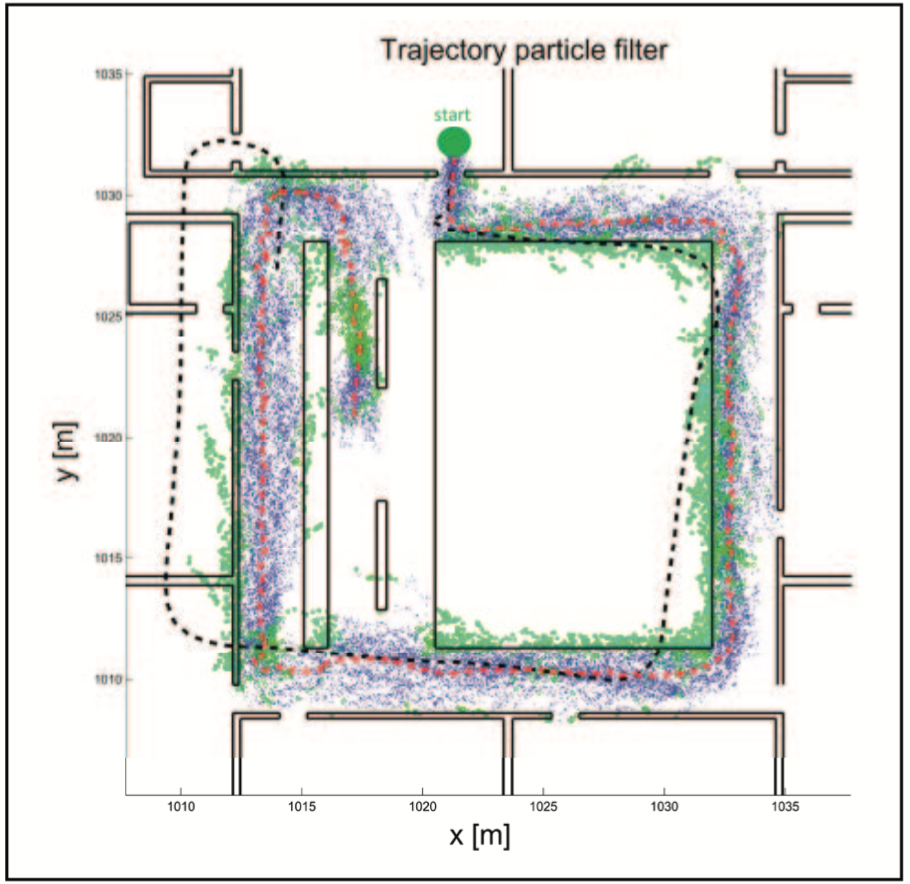
\includegraphics[width=150px]{img/willemsen2014_kalman.png}
            \caption{Objekto kelio spėjimas, panaudojus Dalelių ir Kalman filtrą }
        \end{figure}

    \end{frame}

    \begin{frame}
        \frametitle{Action trajectory reconstruction from inertial sensor measurements \cite{suvorova2012action}}

        Uždavinys: Panaudojus inercinių jutiklių duomenis, nustatyti rankos pozicijos pokyti laike

        Metodai:
        \begin{itemize}
            \item Wavelet transformacija
            \item Residual continuous wavelet transform
        \end{itemize}
    \end{frame}

    \begin{frame}
        \frametitle{Rezultatas}

        \begin{figure}[H]
            \centering
            \subfloat{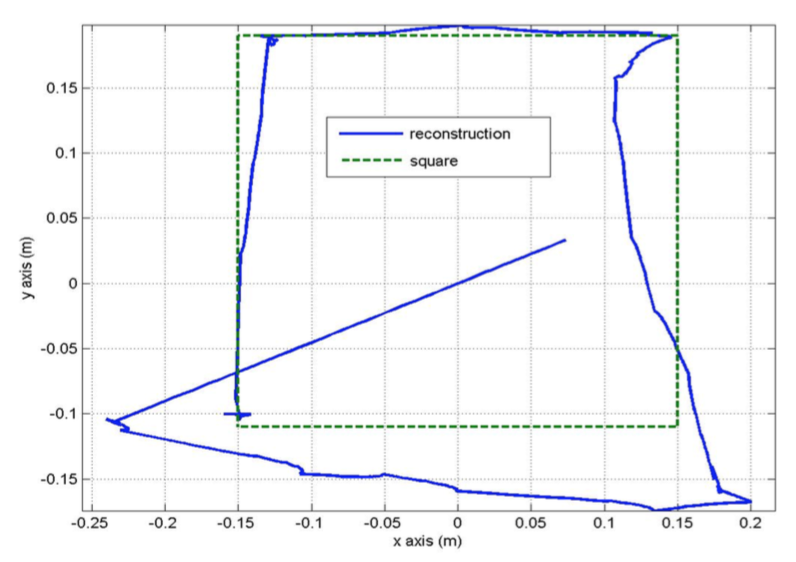
\includegraphics[width=140px]{img/surova_1.png}}
            \subfloat{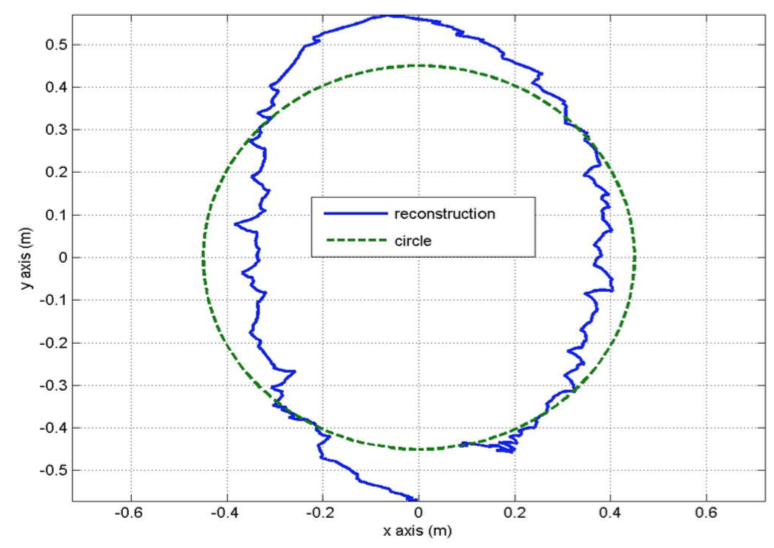
\includegraphics[width=140px]{img/surova_2.png}}
            \caption{Pozicijos pokyčio rekonstrukcija.}
        \end{figure}
    \end{frame}

    \begin{frame}
        \frametitle{Fuzzy logic based 2D position estimation for small robotic fish using low cost MEMS accelerometer \cite{yoo2011fuzzy}}

        Uždavinys: Robotinės žuvies pozicijos nustatymas, panaudojus pigius MEMS jutiklius

        Metodai:
        \begin{itemize}
            \item Least squares algorithm
            \item Fuzzy Logic
            \item Moving average filter
        \end{itemize}
    \end{frame}

    \begin{frame}
        \frametitle{Rezultatas}

        \begin{figure}[H]
            \centering
            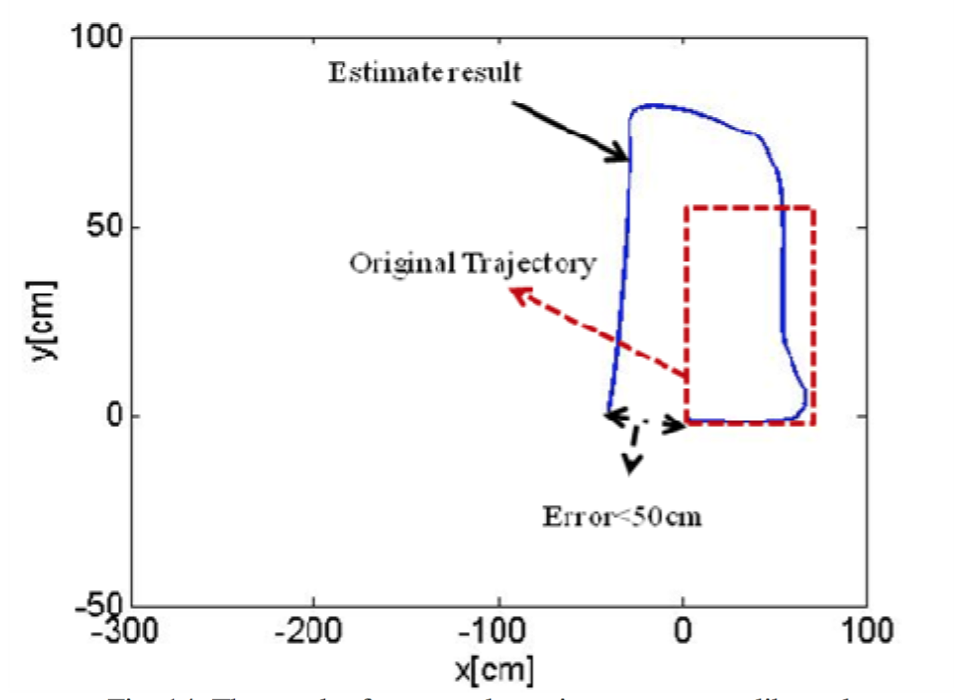
\includegraphics[width=150px]{img/yoo2011_calibrated.png}
        \end{figure}
    \end{frame}

    \begin{frame}   
        \frametitle{Indoor pedestrian navigation using miniaturized low-cost MEMS inertial measurement units \cite{yuan2014indoor}}

        Užduotis: Pristatyti pastato vidaus navigacinę sistemą. Nustatyti geriausią jutiklio poziciją ant žmogaus.

        Metodai:
        \begin{itemize}
            \item Extended Kalman filter
        \end{itemize}

    \end{frame}

    \begin{frame}
        \frametitle{Rezultatai}

        \begin{figure}[H]
            \subfloat{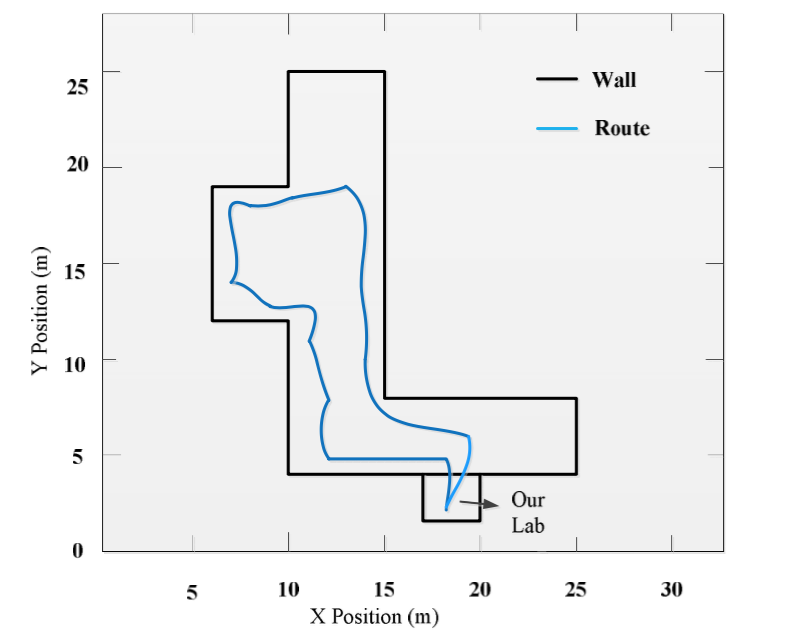
\includegraphics[width=140px]{img/yuan2014_1.png}}
            \subfloat{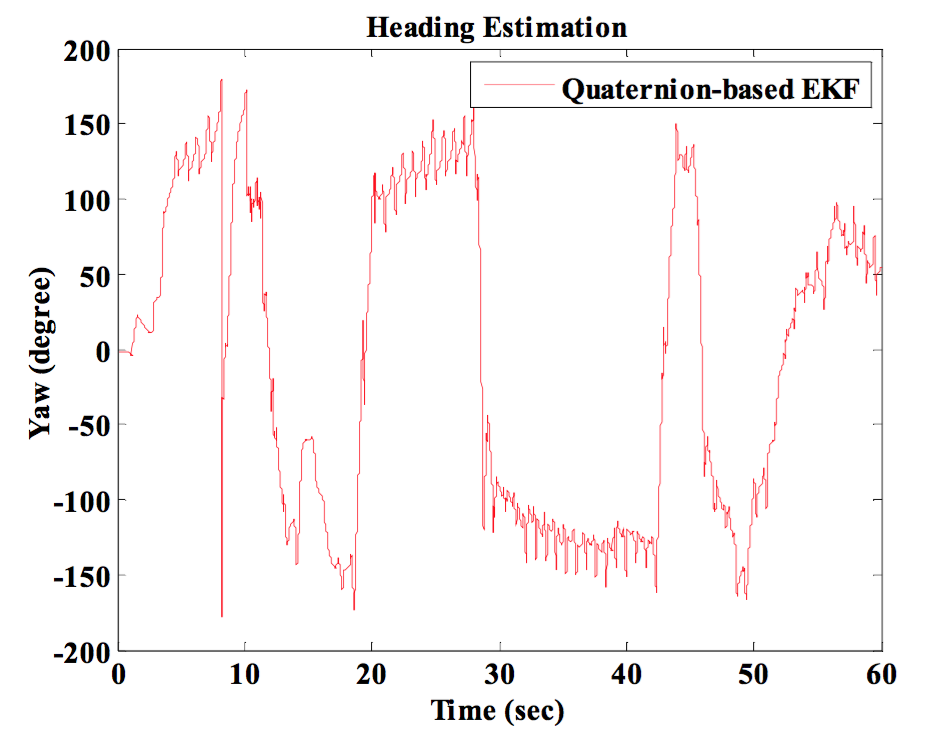
\includegraphics[width=140px]{img/yuan2014_2.png}}
            \caption{Navigacinė sistema sukurta, kuri sugeba nustatyti kryptį}
        \end{figure}
    \end{frame}

    \begin{frame}
        \frametitle{Literatūra}
        
        \bibliographystyle{plain}
        \bibliography{references}
    \end{frame}

\end{document}